\documentclass[conference]{IEEEtran} % Camera-ready format

\usepackage{graphicx}             % import, scale, and rotate graphics
\usepackage{subfig}            % group figures
\usepackage{url}                  % facilitate linebreaking of URLs
\usepackage[latin1]{inputenc}     % use characters with accents in the source
\usepackage{nicefrac}             % write fractions in the text
\usepackage{indentfirst}          % indent the first paragraph
\usepackage[super, negative]{nth}
\usepackage{multirow}
\usepackage{moreverb}
\usepackage{amsmath}
\usepackage{amsfonts}
\usepackage{dcolumn}
\usepackage[dvipsnames,usenames]{color}
\usepackage{xspace}

\usepackage{array,booktabs}
\usepackage{latexsym}
\usepackage{pifont}
\usepackage{colortbl}
\usepackage{bytefield}

\newcommand{\ed}[1]{\textsf{\textbf{[#1]}}}  %editorial comments
\newcommand{\dfn}[1]{\textit{#1}}            %introducing new terms
\newcommand{\revision}[1]{\tr{#1}}
\newcommand{\co}[2]{#1 & \tiny{$\pm#2$}}     %intervalles de confiance
\newcommand{\ttlexceeded}{\texttt{time-exceeded}\xspace}
\newcommand{\tpropagate}{\texttt{ttl-propagate}\xspace}
\newcommand{\echoreply}{\texttt{echo-reply}\xspace}
\newcommand{\echorequest}{\texttt{echo-request}\xspace}
\newcommand{\dstunreach}{\texttt{destination-unreachable}\xspace}
\newcommand{\traceroute}{\texttt{traceroute}\xspace}
\newcommand{\ping}{\texttt{ping}\xspace}

\hyphenation{trace-route trace-routes trace-rout-ing}
\hyphenation{destination-un-reachable dest-ination-unreachable
destination-un-reach-able des-tination-unreachable desti-nation-unreachable
destina-tion-unreachable}
\hyphenation{AS-es}
\hyphenation{Topo-logy}

\graphicspath{{.}{./Figures/}}

\begin{document}

\title{A Funky Title}
\author{Gabriel Davila Revelo{$^{\ddag}$}, Mauricio Anderson Ricci{$^{\ddag}$} , Benoit Donnet{$^{\ast}$},
Jos\'e Ignacio Alvarez-Hamelin{$^{\ddag}$}\\
$\ddag$ Universidad de Buenos Aires, Buenos Aires -- Argentina\\ 
\{gdavila, manderson, ihameli\}@cnet.fi.uba.ar \\
$\ast$ Universit\'e de Li\`ege, Li\`ege -- Belgium\\
\{benoit.donnet\}@ulg.ac.be
}

\maketitle

\begin{abstract}
Recently,  researches have been conducted to discover and assess the usage of
MPLS tunnels.  Indeed, recent developments in the ICMP protocol make certain
categories of MPLS tunnels transparent to \traceroute probing.  Additional
techniques have been proposed to reveal the presence of MPLS tunnels when they
do not explicitly appear in \traceroute.  It has been shown that MPLS is a very
well deployed technology whose usage (i.e., Traffic Engineering, load
balancing, etc.) varies in time and according to ASes.
However, the MPLS structure  on the Internet architecture has not been
studied yet.  In this paper, we follow this path by providing to contributions
to the state of the art: ($i$) we evaluate the biases involved on MPLS tunnel
detection when they are not directly revealed through \traceroute.  ($ii$), we
provide some properties and architectural details related with MPLS deployment
on router topology based on a $k$-core decomposition.
\end{abstract}

\section{Introduction}\label{intro}
% %%%%%%%%%%%%%%%%%%%%%
Internet topology refers to the study of the various types of
connectivity structures and representations between directly connected nodes on
the Internet architecture~\cite{Calvert97}. This representation aims at
obtaining models that represent  Internet with the greatest possible accuracy in order
to test new communications protocols, algorithms, QoS policies, traffic
engineering, etc.

The Internet topology can be seen at several abstraction levels i.e., IP
interface, router, subnetwork, PoP, and Autonomous System (AS) levels. All these
models have been widely studied in the past~\cite{DONNET13} . However, the
current state of the art of Internet deployments involves a great number of
technologies impacting the Internet Topology.  And those technologies deserve a
deep study in order to include them in Internet topology models.  For instance, 
\dfn{Multiprotocol Label Switching} (MPLS)~\cite{rfc3031} has been recently the
focus of several studies~\cite{SOM11,DONNET13,Vanaubel15}.  It has been
demonstrated that MPLS is a mature technology widely deployed for (mainly) load
balancing reasons or traffic engineering purposes.  Although few studies have
partially questioned its impact on Internet topology~\cite{BRICE07,Flach2012}, the impact of MPLS deployment on the Internet architecture has not been
studied yet in deep. The importance to study new architectural details, structure and topological
features related with MPLS usage would help to know the way in
which the Internet Service Providers (ISPs) use their networks or apply their
policies for traffic engineering as well as to better understand the today's
Internet architecture more accurately. Our work provides a study around the
impact of MPLS deployments over Internet Topology. Principally, we focus on the
bias involved in MPLS tunnel detection and on the features that MPLS modifies over traditional networks maps such as router level topology. For our purpose, we mainly based on  $k$-core
decomposition method~\cite{batagelj2002}. In this way, it has been shown
previously that the $k$-core decomposition is a relevant tool to describe
Internet Topology ~\cite{Alvarez06k, Serrano06, Serrano06, Alvarez08k}.

This paper adds complementary information around MPLS
usage on Internet. First, we present a quantification of the biases involved on
implicit MPLS tunnel detection. Additionally, we provided some properties and
architectural details related with MPLS deployment on router level topology. We found
that routers are commonly connected to  MPLS
networks. Finally, we found that ASes seems to have different MPLS structure 
according the type of MPLS tunnel that prevails.


The remainder of this paper is organized as follows: Sec.~\ref{related} provides
the state of the art and the background related to MPLS tunnels discovery. In
particular, it describes how MPLS tunnels can be revealed through active
measurements;  Sec.~\ref{dataset} explains how we collected data for this work;
Sec.~\ref{validation} presents our results related to \textit{mpls signatures}
accuracy; Sec.~\ref{cluster} presents the main contributions of this paper with
a detailed study around the behaviour of MPLS networks on the Internet Topology
and architectural details of some ASes with most MPLS usage; Finally,
Sec.~\ref{ccl} concludes this paper by summarizing its main achievements.


\section{Related Work}\label{related}
% %%%%%%%%%%%%%%%%%%%%
In this section, we first provide an overview of MPLS
(Sec.~\ref{related.overview}) before explaining how MPLS tunnels can be revealed
through active measurements (Sec.~\ref{related.revealing}).  We also position
this work regarding the state of the art.

\subsection{MPLS Overview}\label{related.overview}
%%%%%%%%%%%%%%%%%%%%%%%%%%%
The \dfn{Multiprotocol Label Switching} (MPLS)~\cite{rfc3031} was originally
designed to speed up the forwarding process. In practice, this was done with one
or more 32 bits \dfn{label stack entries} (LSE) inserted between the frame
header (Data-link layer) and the IP packet (Network layer).\footnote{MPLS is IP
layer protocol independent.} A given packet can manage several LSEs at the same
time. In this case, the packet is said having a \dfn{stack of labels}.  Each LSE
is made of four fields:  a 20-bit label value used for forwarding the packet to
the next router, a 3-bit Traffic Class field for quality of service (QoS),
priority, and Explicit Congestion Notification (ECN)~\cite{rfc5462}, a 1-bit
bottom of stack flag (when set the current label is the last in the
stack~\cite{rfc3032}), and an 8-bit time-to-live (LSE-TTL) field having the same
purpose as the IP-TTL field~\cite{rfc3443}.

MPLS routers, called \dfn{Label Switching Routers} (LSRs), exchange labelled
packets over \dfn{Label Switched Paths} (LSPs).   The first MPLS router
(\dfn{Ingress Label Edge Router}, or Ingress LER, i.e., the tunnel entry point)
adds the label stack, while the last MPLS router (\dfn{Egress Label Edge
Router}, or Egress LER, i.e., the tunnel exit point) removes the label stack.
In some cases, for performance reasons, the LSE stack may be removed by the
penultimate MPLS router (\dfn{penultimate hop popping}, PHP).  The Egress LER
then performs a classic IP lookup and forwards the traffic, reducing so the load
on the Egress LER (specially if the Egress LER is shared among several LSPs).
This means that, when using PHP, the tunnel exit is one hop before the Egress
LER. % In its most basic operation, LSPs are constructed along best effort routes
%using the \dfn{Label Distribution Protocol} (LDP~\cite{rfc5036}). More specific
%LSPs may be constructed for Traffic Engineering purposes, using an extension of
%the RSVP protocol, \dfn{RSVP-TE}~\cite{rfc3209}. In these two cases, the label
%stack contains only one LSE. A more complex usage is for Virtual Private Networks
%(VPN~\cite{rfc2917}), where LSPs are constructed using either LDP or RSVP-TE,
%and an additional LSE at the bottom of the label stack is used to specify a Virtual
%Routing Table at the Egress. In this case, the bottom of the stack is constant
%along an LSP, while the top of the stack is modified at each hop, as in the
%previous cases.

\subsection{Revealing MPLS Tunnels}\label{related.revealing}
% %%%%%%%%%%%%%%%%%%%%%%%%%%%%%%%%%%
MPLS routers may send ICMP \ttlexceeded messages when the LSE-TTL expires. In
order to debug networks where MPLS is deployed, routers may also implement
RFC4950~\cite{rfc4950}, an extension to ICMP allowing a router to embed an MPLS
LSE in an ICMP \ttlexceeded message. In that case, the router simply quotes the
MPLS LSE (or the LSE stack) of the received packet in the ICMP \ttlexceeded
message. RFC4950 is particularly useful for operators as it allows them to
verify the correctness of their MPLS tunnels and TE policy.

If the Ingress LER copies the IP-TTL value to the LSE-TTL field rather than
setting the LSE-TTL to an arbitrary value such as 255, LSRs along the LSP will
reveal themselves when using \traceroute via ICMP messages even if they do not
implement RFC4950. Operators can configure this action using the \tpropagate
option provided by the router manufacturer~\cite{rfc3443} (while, to the best of
our knowledge, the RFC4950 is just a matter of implementation and cannot be
deactivated on recent routers supporting it). 

Using those two features, Sommers et al.~\cite{SOM11} provide an extensive study
of MPLS tunnels as observed in CAIDA's topology data.  In this data, they find
tunnels in 7\% of ASes, and the fraction is constant over the years of data
considered.  In addition, Sommers et al. propose a statistical methodology to
infer MPLS tunnels in archived data where ICMP extensions are not recorded.
Vanaubel et al.~\cite{Vanaubel15} propose a classification of path diversity
according to MPLS deployment.  Their classification reveals the actual usage of
MPLS (e.g., load balancing, traffic engineering) according to the inferred label
distribution protocol.  Finally, it has also been demonstrated that MPLS tunnels
may have an impact on Internet topology discovery tools.  For instance, the
presence of MPLS tunnels may interfere with load balancing
detection~\cite{BRICE07} or violate the destination-based
forwarding~\cite{Flach2012}.

Donnet et al.~\cite{Donnet12} propose a taxonomy of MPLS tunnels based on how
they react to \traceroute probes according to their compliance (or not) to
RFC4950 for MPLS and the \tpropagate option.  The classes proposed are:
\dfn{explicit tunnels} (i.e., \tpropagate and RFC4950 are enabled),
\dfn{implicit tunnels} (i.e., the router that pushes the MPLS label enables the
\tpropagate option but LSRs do not implement RFC4950), \dfn{opaque tunnels}
(i.e., the LH implements RFC4950 but the ingress LER does not enable the
\tpropagate option), and, finally, \dfn{invisible tunnels} (i.e., the ingress
LER does not enable the \tpropagate option and RFC4950 is not implemented by the
LH router).  Implicit and opaque tunnels can be revelead as follows:
\begin{enumerate}
  \item a quoted IP-TTL (\dfn{qTTL}) in ICMP \ttlexceeded messages $>1$ will
  likely reveal the \tpropagate option at the ingress LER of an LSP. For each
  subsequent \traceroute probe within an LSP, the qTTL will be one greater
  resulting in an increasing sequence of qTTL values in \traceroute.  This is
  illustrated in Fig.~\ref{validation.qTTLFig};
  \item  \#hops differences with the IP-TTL in \echoreply messages
  (\dfn{u-turn}).  It relies on the fact that LSRs along an LSP present an
  \textit{original label stack} default routing behavior: when the LSE-TTL
  expires, an LSR first sends the \ttlexceeded reply to the Egress LER which
  then forwards the reply on its own to the probing source, while an LSR
  replies to other probes using its own IP routing table if available. Summarizing, 
  $\textit{u-turn}=\text{TTL}_{\text{echo-reply}}-\text{TTL}_{\text{time-exceeded}}$.
  The expected u-turn value is in the form $[2L, 2L-2, 2L-4,..., 2]$ where $L$
  is the tunnel length and the array position corresponds to the LSR position
  within the LSP.
  \item opaque tunnels are revealed through an \textit{abnormal} LSE-TTL
  ($1<$LSE-TTL$<255$) returned by the LH in the \ttlexceeded reply.
\end{enumerate}

Additional study by Vanaubel et al.~\cite{VAN2013} shows that the probing
heuristic to detect implicit tunnels seems quite reliable.  However, u-turn
signatures are by definition more subject to false positives than qTTL ones. 
This is exactly what we tackle in this paper (and, consequently, our work is
complementary to Vanaubel et al.~\cite{VAN2013}): we want to test u-turn
signature accuracy.

%Figura u-turn
% \begin{figure*}[!t]
%   \begin{center}
%     \subfloat[Tunnel Length Distribution]{\label{hist_length}
%       \includegraphics[width=6cm]{hist_length}}
%       \hfil
%     \subfloat[\textit{qTTL} and $n$-position comparison]{\label{n_vs_qttl}
%       \includegraphics[width=6cm]{n_vs_qttl}} 
%       \hfil
%     \subfloat[\textit{u-turn} on LSRs revealed through RFC4950 and \textit{qTTL}]{\label{fig_uturn_a}
%       \includegraphics[width=6cm]{n_vs_uturn_L5_exp}}
%       \hfil
%     \subfloat[\textit{u-turn} on LSRs where no other signature was found]{\label{fig_uturn_b}
%       \includegraphics[width=6cm]{n_vs_uturn_L5}}
%    \end{center}
%   \caption{ Comparison between obtained and expected values for \textit{qTTL} and
%   \textit{u-turn} signatures. On figures (b), (c) and (d) the circle size in the scatter plot is related with the occurrence frequency of \textit{y-axis} values regarding each $n$-position. The
%   transparency of the circle is related with occurrence frequency of $n$-position  regarding each \textit{y-axis} value, e.g., on figure (b) for values where $n>1$, the biggest circles are mainly located on  $\textit{qTTL}=1$ and $\textit{qTTL}=n$ so this suggest that for a given $n$-position the \textit{qTTL} value usually takes either the value of $1$ or $n$; in the same way, the transparency value suggests that for a given \textit{qTTL} value the $n$-position usually takes the same \textit{qTTL} value.  \textbf{Figure (c)} and \textbf{Figure (d)} suggest that \textit{u-turn} value is overestimated. }
%   \label{ig_signatures}
% \end{figure*}

% \section{Related Work}\label{related}
% %%%%%%%%%%%%%%%%%%%%
% In the last years, MPLS~\cite{rfc3031} has been more and more investigated by
% the researchers.  This works mainly focused on MPLS tunnels detection. For
% instance, \Sommers et al.~\cite{SOM11} studied the MPLS deployment that is
% explicitly revealed through \textit{RFC 4950} extension. They also
% proposed a methodology to infer MPLS tunnels in archived data where ICMP extensions are not
% recorded. Most recently Donnet et al.~\cite{Donnet12} provided a
% taxonomy for MPLS tunnels and propose algorithms for detecting MPLS tunnels
% depending on the way that the LSRs react to the \textit{ttl-propagate} and
% \textit{RFC 4950} options. \ed{BD: I would remove this paragraph as it
% introduces concepts (RFC4950, LSRs, \ldots) that have not been }
% 
% It has also been studied the path diversity related with MPLS deployments. In
% this way, \textit{Vanaubel et al.} \cite{Vanaubel15} recently proposed and
% algorithm to better understand the path diversity and their usage within a given
% AS.
% 
% In this way, our work is complementary to tunnel detection issues. We test
% carefully some of the ways that reveals  MPLS tunnels and provided an analysis
% of how the MPLS tunnels impact the Internet Topology structure.

% \subsection{MPLS overview}\label{related.mpls}
% % %%%%%%%%%%%%%%%%%%%%%%%%% 
% MPLS \cite{RFC3031} was originally designed
% to speed up the forwarding process. In practice, this was done with one or more
% 32 bits Label Stack Entries (LSE) inserted between the frame header  and the IP
% packet.
% 
% In a MPLS network, packets are forwarded using an exact match lookup of a 20-bit
% label found in the LSE. An MPLS LSE also has a Time-To-Live (TTL) called LSE-TTL
% field and a Type-of-Service (ToS) field \cite{rfc1771}. At each MPLS hop, the
% label of the incoming packet is replaced by a corresponding outgoing label found
% in an MPLS switching table. A portion of a path where the forwarding decision is
% not anymore based on longest prefix matching but rather on MPLS features is
% known as an MPLS tunnel. A router with label switching capabilities is called
% Label Switching Router (LSR). A series of LSRs connected together form a Label
% Switched Path (LSP). The first router where the incoming packet includes a LSE
% is called ingress Label Edge Router (LER) and the last router that \textit{pops}
% the LSE is called Last Hop (LH).

% \subsection{Revealing MPLS tunnels} \label{related.signatures}
% 
% \textit{Donnet et al.} \cite{Donnet12} provided a taxonomy for MPLS tunnels
% revealed by traceroute and developed algorithms in order to detect it based on
% the way that LSR react to \textit{ttl-propagate}  and \textit{RFC 4950} option.
% Basically, their proposes two kind of visible MPLS tunnels: explicit tunnels and
% implicit tunnels.
% 
% Explicit tunnels are based on \textit{RFC 4950} implementation. MPLS routers may
% send ICMP time-exceeded messages when the LSE-TTL expires. The \textit{RFC 4950}
% is an extension to ICMP allowing a router to embed an MPLS LSE in an ICMP
% time-exceeded message. In that case, when the LSE-TTL expires on a MPLS router,
% it simply quotes the MPLS label stack in the ICMP \textit{time-exceeded}
% message.
% 
% Implicit tunnels discovery are based on two signatures detection: \textit{qttl}
% and \textit{u-turn} signature. The \textit{qttl} signature is relate with
% \textit{ttl-propagate} option. If  \textit{ttl-propagate} is implemented the LER
% copies the IP-TTL value to the LSE-TTL field rather than setting the LSE-TTL to
% an arbitrary value such as 255. In this way, the LSRs along the LSP will reveal
% themselves via ICMP messages even if they do not implement \textit{RFC 4950},
% i.e., if $\textit{qttl}>1$  the ICMP message was generated by an interfaces that
% belongs to an MPLS tunnel. The \textit{u-turn} signature relies on the fact that
% most LSRs in an LSP present a common behaviour: when the LSE-TTL expires, the
% LSR sends the ICMP \textit{time-exceeded} message to the LH router which then
% forwards the reply to the probing source, while an LSR replies to other probes
% such as  ICMP \textit{echo} packets using directly its own IP routing table if
% available. The variation between these two TTLs values is called \textit{u-turn}
% signature, i.e.,
% $\textit{u-turn}=TTL_{\text{echo-reply}}-TTL_{\text{time-exceeded}}$.  The
% expected \textit{u-turn} value in the form $[2L, 2L-2, 2L-4,..., 2]$ where $L$
% is the tunnel length and the array position correspond to the LSR position
% within the tunnel.
% 
% The \textit{qttl} signature ($\textit{qttl}>1$) is present just in MPLS
% behaviour.
% Commonly there is not another way to get a $\textit{qttl}>1$. However,
% \textit{u-turn} signature could be caused for another Internet issues such as
% police routing or load balancing paths, that produces different lengths in the
% return path.

% In this paper we consider that \textit{RFC 4950} implementation and
% \textit{qttl} signature are highly reliable methods to reveal MPLS tunnels and
% we mainly focus on to test \textit{u-turn} signature accuracy.

% \subsection{Diversity on MPLS paths}
% 
% \textit{Vanaubel et al.} \cite{SOM11} proposed a classification of path
% diversity on MPLS deployments. Their algorithm allow to classify the kind of
% diversity path regarding the behaviour of mpls labels on explicit tunnels. The
% authors propose basically a path classification based on physical diversity
% i.e., paths with different IP interfaces; and logical diversity i.e., paths with
% the same IP interfaces but different labels. The work show a detailed study of
% path diversity over the top of ASs with most MPLS tunnels discovered.       

\section{Dataset}\label{dataset}

Because part of our works focus on signature validation, we developed our own
measurement tool in order to get \textit{qTTL} and \textit{u-turn} signatures.
We use \textit{Magallanes} [REF] which is an open source software that allows
to run and to manage Scamper \cite{Luckie10} based probes through Planet Lab (PL) infrastructure. \textit{Magallanes}  allocates randomly several Vantage Points (VP) within the available set of PL nodes and it distributes a given number of destination  targets to each VP. To achieve uniformity in target selection,  \textit{Magallanes} uses data provided by MaxMind\footnote{\url{www.maxmind.com}}. In this way, it chooses the targets randomly and proportionality distributed according to the number of subnets assigned by the Regional
Internet Registry (RIR) to each region. Additionally, it allows to storage the experiments results on a centralized database and to solve alias resolution process using MIDAR \cite{Keys13}. 

For our experiment, we run the exploration October 31, 2015. We choose 100 VP and we selected 10K of destination targets per VP. Each set of destination targets are disjoint sets. We use ICMP-Paris probes  in order to avoid load balancing issues in
the forwarding path. To get the \textit{u-turn} signature, we send a
\textit{ping} to each hop revealed by traceroute. We sent six ICMP-echo packets
from the same monitor. Six ICMP-echo responses allows us to infer with $95\%$
confidence if there is a single return path length and therefore reduce
measurement error caused by a reverse path containing load-balanced segments of
different lengths \cite{BRICE07}. As a result we discovered around 270K of IP interfaces 520K links, $42\%$ of which were available to run MIDAR and we found aliases successfully on $19\%$ of then. To match IP interfaces to ASes, we use the RouteViews Dataset provided by CAIDA.  Additionally
we found MPLS tunnels on  $44\%$ of the traceroutes. The amount of explicit
tunnels is highly superior to implicit tunnels. We discovered explicit tunnels
on $34\%$ of traceroutes and at least one implicit tunnel on $16\%$.
Surprisingly we found more implicit tunnels revealed through \textit{u-turn}
signature ($12\%$) rather than \textit{qTTL} signature ($4\%$). However, the \textit{qTTL} signature match with at least $63\%$ of the explicit tunnels. We discuss these
results in the next sections. Finally, we did not found opaque tunnels.

\section{MPLS Signatures Validation}\label{validation}
% %%%%%%%%%%%%%%%%%%%%%%%%%%%%%%%%%%%%

%Figura u-turn
\begin{figure*}[!ht]
  \begin{center}
    \subfloat[Tunnel Length Distribution]{\label{hist_length}
      \includegraphics[width=6cm]{hist_length}}
      \hfil
    \subfloat[\textit{qTTL} and $n$-position comparison]{\label{n_vs_qttl}
      \includegraphics[width=6cm]{n_vs_qttl}} 
      \hfil
    \subfloat[\textit{u-turn} on LSRs where no other signature was found]{\label{fig_uturn_a}
      \includegraphics[width=6cm]{n_vs_uturn_L5}}
      \hfil
    \subfloat[\textit{u-turn} on LSRs revealed through RFC4950 and \textit{qTTL}]{\label{fig_uturn_b}
      \includegraphics[width=6cm]{n_vs_uturn_L5_exp}}    
  \end{center}
  \caption{ Comparison between obtained and expected values for \textit{qTTL} and
  \textit{u-turn} signatures. On figures (b), (c) and (d) the circle size in the scatter plot is related with the occurrence frequency of \textit{y-axis} values regarding each $n$-position. The
  transparency of the circle is related with occurrence frequency of $n$-position  regarding each \textit{y-axis} value, e.g., on figure (b) for values where $n>1$, the biggest circles are mainly located on  $\textit{qTTL}=1$ and $\textit{qTTL}=n$ so this suggest that for a given $n$-position the \textit{qTTL} value usually takes either the value of $1$ or $n$; in the same way, the transparency value suggests that for a given \textit{qTTL} value the $n$-position usually takes the same \textit{qTTL} value. This suggest that \textit{qTTL} highly match with $n$-position.  \textbf{Figure (c)} and \textbf{Figure (d)} suggest that \textit{u-turn} value is overestimated. }
  \label{ig_signatures}
\end{figure*}

In this section we describe the used methodology to validate the MPLS signatures
revealed by traceroutes. As we described previously, the RFC9450 and
\textit{qTTL} signature are fingerprints that occurs just on MPLS behaviour,
while \textit{u-turn} could be related with issues not related with MPLS such as
load balancing. Thereby we mainly focus on test the \textit{u-turn} signatures.

If the RFC4950 is not implemented in the LSRs, the only way to reveal
an MPLS tunnel is trough \textit{qTTL} or \textit{u-turn} signatures. Both of
them are directly related with the position of MPLS within the tunnel:

\begin{itemize}
  \item[i] \textit{qTTL} value refers to the TTL of ICMP-\textit{echo}
  message when it enters to the MPLS  tunnel. A quoted TTL of $n$ in
  the incoming ICMP reply means that the sent probe
  expired $n$ hops later to ingress to the \textit{LSP}. In this way, we can say
  that a LSR that replies with $\textit{qTTL}=n$ appears  in the $n$ position of
  MPLS tunnel.
  \item[ii] The expected \textit{u-turn} value is related with the tunnel length and the position of the LSR within the tunnel (see section \ref{related.revealing})
\end{itemize}


%\begin{figure*}[!t]
%\centering
%\subfloat[Case I]{\includegraphics[width=2.5in]{box}%
%\label{fig_first_case}}
%\hfil
%\subfloat[Case II]{\includegraphics[width=2.5in]{box}%
%\label{fig_second_case}}
%\caption{Simulation results for the network.}
%\label{fig_sim}
%\end{figure*}

Our signature validation relays on the hypothesis that the MPLS position match
with the $n$-position  which an LSR is revealed by traceroute. Indeed,
we use a paris-traceroute \cite{BRICE06}  based tool in order to sure that the probes follow the
same path. In order to validate our hypotheses we first filter  tunnels revealed by \textit{u-turn} signature and we test our hypothesis on explicit tunnels and tunnels revealed by \textit{qTTL} signatures. Thereby we remove the bias caused by possible false
\textit{u-turn} signatures. The \textit{qTTL} values of our dataset  should to match with
$n$-position to validate our assumption, i.e., $\textit{qTTL}=n$.

The figure \ref{hist_length} shows the MPLS tunnel length distribution found in our dataset. Additionally,  we compare the \textit{qTTL} value and their respective $n$-position revealed by traceroute. The
results are showed in figure \ref{n_vs_qttl}. We noticed that \textit{qTTL}
signature highly match with the $n$-position, i.e., $q\textit{ttl}=n$.  A bias could
occur due to the limitation in our method to reveal the first LSRs in
the tunnel if it does not implement the RFC4950. %, i.e., the first LSR revealed by traceroute within the tunnel  ($n=1$) could correspond to a LSR with $\textit{qTTL}>n$. 
A second deviation
occurs due to possible load balancer presence in the follow path. In this case,
the traceroute probes follow paths with different lengths before to reach the
MPLS tunnel. This issue
produce that the same \textit{qTTL} value could be revealed many times in different
$n$-positions. The figure also shows that \textit{qTTL} 
takes frequently the value of $1$. This usually  means that \tpropagate is not implemented. However, we found that around $2\%$ of LSRs do not react to \textit{qTTL} signature, even if \tpropagate option is activated on the tunnel, i.e., some LSRs interfaces located at $i_{n-1}$  and $i_{n+1}$ tunnel positions have valid \textit{qTTL} signatures but the LSR interface located at $i_n$ position does not. We think that this issue occurs because some
routers update the IP-TTL to $1$ in the expired packet instead of keeping it
unchanged as usual. We found that in $58\%$ of the cases the $n$-position match with the
\textit{qTTL} value while in $36,3\%$ of cases the \textit{qTTL} signature is not
present and takes the value of $1$, and just $6,7\%$ of the cases presented
some bias around the expected value.

Once we proved  that \textit{qTTL} highly match with  $n$-position, we use
this position as a reference value to validate the \textit{u-turn} signature. In
this case, the expected value should to be $\text{u-turn}=2(L-(n-1))$ where $n$ is the
position of the LSR within the tunnel (particularity \textit{qTTL} value) and $L$ is the tunnel length. Because
\textit{u-turn} is commonly present in almost all LSRs, first we tested it in
MPLS tunnels  where other signatures were found, i.e., LSRs revealed
through RFC4950 and \textit{qTTL} signatures.
Secondly, we tested it on LSRs where \textit{u-turn} was the only
signature that allows us to reveal the MPLS tunnel. We use the filter ($\textit{u-turn}>3$) to
avoid false isolated \textit{u-turn} signatures. We compare the expected values and the
obtained values using a scatter plots in order to distinguish the amount of
signatures biased. The results for a given length are showed in figures
\ref{fig_uturn_a}, \ref{fig_uturn_b}. The same results were showed for other length values. Basically, we noticed that the obtained values are close to expected values either on LSRs revealed explicitly and through \textit{qTTL} signature (figure \ref{fig_uturn_a}). However on the set of  LSRs revealed just by \textit{u-turn} signatures (figure \ref{fig_uturn_b}) the values does not match. If we accept a bias of $ \pm 2$ around the expected value, we
noticed that on LSRs revealed through RFC4950 implementation and
\textit{qtll} signatures, the $60\%$ of obtained \textit{u-turn} values match
with the expected values. However, on LSRs
where no other signature was obtained (therefore where the \textit{u-turn} signature
is really useful), the obtained \textit{u-turn} signature just match in $25\%$. 
Therefore, we conclude that the LSRs revealed through \textit{u-turn}
signatures are highly overestimated. Mainly because MPLS tunnels are not the
only behaviour that could causes \textit{u-turn} signatures. Indeed, has been showed that load balancing is present in almost $39\%$ of traverse paths even between the same pairs source-destination \cite{BRICE07}. This issue is called \textit{per-flow} load balancing. Basically, packets that belongs to the same \textit{flow} are treated similarly \cite{BRICE06}. A \textit{flow} is identified by the first 32 bits of the IP \textit{payload}. In the case of ICMP messages, this fields refers to \textit{Type},
\textit{Code} and \textit{Checksum}. By definition, \textit{u-turn} signature is
based on two kinds of ICMP messages: ICMP \echoreply \textit{Code 11} and ICMP
\ttlexceeded \textit{Code 0}. Due to the different codes values
related with each ICMP message, there is no way to sure that they belong to the same \textit{flow} identifier and thereby to be sure that \textit{u-turn} value is caused just by MPLS tunnels.

\section{LSRs and \textit{MPLS clusters}}\label{cluster}
% %%%%%%%%%%%%%%%%%%%%%%%%%%%%%%%%%%%%%%
To the best of our acknowledge, MPLS interconnection architecture on Internet
topology has not yet been studied. In this way, we focus our attention on
studying several LSRs properties and \dfn{MPLS clusters} (i.e., set of MPLS
graphs) and their interactions with non MPLS networks. Our study aims at better
understanding the impact of MPLS deployments over Internet, specifically over
router level topology.

\subsection{Definitions and Background}\label{cluster.methodo}
% %%%%%%%%%%%%%%%%%%%%%%%%%%%%%%%%%%%%%%
\begin{figure*}[!htb]
  \begin{center}
    \subfigure[Degree Distribution Probability]{\label{fig_degree_distribution}
      \includegraphics[width=5.5cm]{DegreeDistribution}}\hfil
    \subfigure[Clustering Coefficient]{\label{fig_clustering}
      \includegraphics[width=5.5cm]{ClusteringCoeficient}}\hfil
    \subfigure[Neighbor Degree Distribution]{\label{fig_neighbor}
      \includegraphics[width=5.5cm]{NearestNeighbor}}
  \end{center}
\caption{Metrics for IP, router and MPLS cluster interconnection
topologies.} 
\label{fig_metrics}
\end{figure*}

\begin{table}[!t]
  \begin{center}
    \begin{tabular}{l|ll}
    \textbf{Graph} & \textbf{Notation} & \textbf{Definition}\\
    \hline
    IP                 & $G_{ip}$ & $(V_{ip}, E_{ip})$\\
    Router             & $G_r$ & $(V_r, E_r)$\\    
    MPLS               & $G_r^{mpls}$ & $(V_r^{mpls}, E_r^{mpls})$\\
    ASes induced graph & $G_r(as)$ & $(V_r(as), E_r(as))$\\    
    MPLS cluster       & $C_i^{mpls}$ & /\\
    MPLS cluster interconnection graph & $G_{r \backslash lsr}$ & $(V_{r
    \backslash lsr}, E_{r \backslash lsr}^{mpls})$
    \end{tabular}
  \end{center}
  \caption{Summary of graph notations used in Sec.~\ref{cluster}.}
  \label{cluster.table_notations}
\end{table}

We defined several graphs at different abstraction levels as follows (they are
summarized in Table~\ref{cluster.table_notations}): The \dfn{IP level graph} is
defined as $G_{ip}=(V_{ip}, E_{ip})$, where $V_{ip}$ is the IP addresses
discovered in our exploration and $E_{ip}$ the set of the links found trough
\traceroute.   Second, the \dfn{router level graph} is defined as $G_{r}=(V_{r},
E_{r})$, where $V_{r}$ is the set of routers (alias resolution having been done
through MIDAR~\cite{Keys13}), and $E_{r}$ is the set of all the links found
between any pair of routers $v \in V_{r}$. Third, the \dfn{MPLS router level
graph} refers to $G^{mpls}_{r}=(V^{mpls}_{r}, E^{mpls}_{r})$ where
$V^{mpls}_{r}$ is the set of routers in which at least one IP interface belongs
to an LSP, and  $E^{mpls}_{r}$ is the set of all \textit{mpls links}
$(v^{mpls}_{r}(i), v^{mpls}_{r}(j))$ such as
$\{{v^{mpls}_{r}(i)},{v^{mpls}_{r}(j)} \}\in V^{mpls}_{r}$.

The \dfn{ASes induced graph} is defined as $G_{r}(as)=(V_{r}(as), E_{r}(as))$.
Each vertex in $G_{r}(as)$ has an interface belonging to the same Autonomous
System, $as$.  In particular, the induced graph of $G_r^{mpls}$ is
$G^{mpls}_{r}(as)=(V^{mpls}_{r}(as), E^{mpls}_{r}(as))$.  This definition allows
us to define an \dfn{MPLS cluster}, $C^{mpls}_{i}$, as a connected component $i$
of $G^{mpls}_{r}(as)$. A given AS may have several MPLS clusters.

Finally, the \dfn{MPLS cluster interconnection graph} is an hybrid router level
graph,  $G_{r\backslash lsr}=(V_{r\backslash lsr},E^{mpls}_{r\backslash lsr})$,
where all the MPLS clusters $C^{mpls}_{i}$ are gathered together in a single
node $v\in V_{r\setminus ls}$, while non-MPLS capable routers remain unchanged.
Broadly speaking, an MPLS cluster interconnection graph refers to a router level
graph where all MPLS clusters are treated as a single node. In this way, we can
study how IP interfaces and non MPLS capable routers interact with MPLS
clusters. Additionally, we call $G_{r\backslash lsr}(as)$ to the induced
subgraphs of $G_{r\backslash lsr}$ by routers having at least one interface in
the Autonomous System $as$.

% \textbf{IP level Graph:} $G_{ip}=(V_{ip}, E_{ip})$, where $V_{ip}$ is the IP
% address discovered in our exploration and $E_{ip}$ is the set of the links found
% trough traceroute. Note that \traceroute just records incident IP addresses in
% a path.

As the analysis is mainly based on $k$-core decomposition, we present the
following definitions:
\begin{itemize}
  \item\dfn{\textit{k}-core:}. Given a graph $G=(V,E)$, then the
  subgraph $H=(C,E|C)$ induced by the set $ C\subseteq V$ is a \textit{k}-core
  of order $k$ $iff$ $\forall v \in C: degree_{H}(v)\geq k$ and $H$ is the
  maximum subgraph with this property.
%A \textit{k}-core of $G$ can therefore be obtained by recursively removing all
% the vertices of degree less than $k$, until all vertices in the remaining
% graph have at least degree $k$.    
  \item\dfn{Shell index}. A vertex $i$ has a shell index $c$ if it
  belongs to the $c$-core but not to $(c+1)$-core. We denote by $C_i$ the shell
  index of vertex $i$. A shell $C_c$ consists of all the vertices whose shell
  index is $c$. The maximum value $c$ such that $C_c$ is not empty is denoted by
  $C_{\max}$.  Therefore, the $k$-core is thus the union of all shells $C_c$ with
  $c \geq k$.
\end{itemize}

To retrieve the $k$-core decomposition of a graph $G$, we use
\lanet\cite{Alvarez06k}.  This tool returns a two dimensional plot,
where the position of each vertex depends on its shell index and its neighbors'
index. A color code allows for the identification of shell indices, while the
vertex's original degree is provided by its size \ed{size of what?  circles on
Fig.~\ref{fig_k_core_MPLS} for instance?}, which depends logarithmically on the
degree. A central role in the visualization method is played by multi-components
representation of $k$-cores.  \ed{It is unclear to me what's a multi-component
representation.  The next sentences in this paragraph are also unclear} In the
most general situation, the recursive removal of vertices having degree less
than a given $k$ can break the original network into various connected
components, each of which might even be once again broken by the subsequent
decomposition.

In this paper, we use $k$-core decomposition focused on properties around mpls
clusters interconnection.  \lanet is useful to read basic features of the graph
(degree, hierarchical structure, etc.) as well as more entangled features, e.g.,
the relation between a vertex and the hierarchical position of its neighbors. It
is also useful to  discriminate between networks with different topological
properties and structural arrangement. This provides us an idea about the
structural arrangement and topological properties caused by MPLS usage.
Additionally, the visualization helps us to find properties and fingerprints
tightly related with MPLS presence.

\subsection{MPLS on Internet Topology}\label{cluster.topo}
% %%%%%%%%%%%%%%%%%%%%%%%%%%%%%%%%%%%%%%
\begin{figure}[!t]
  \begin{center}
    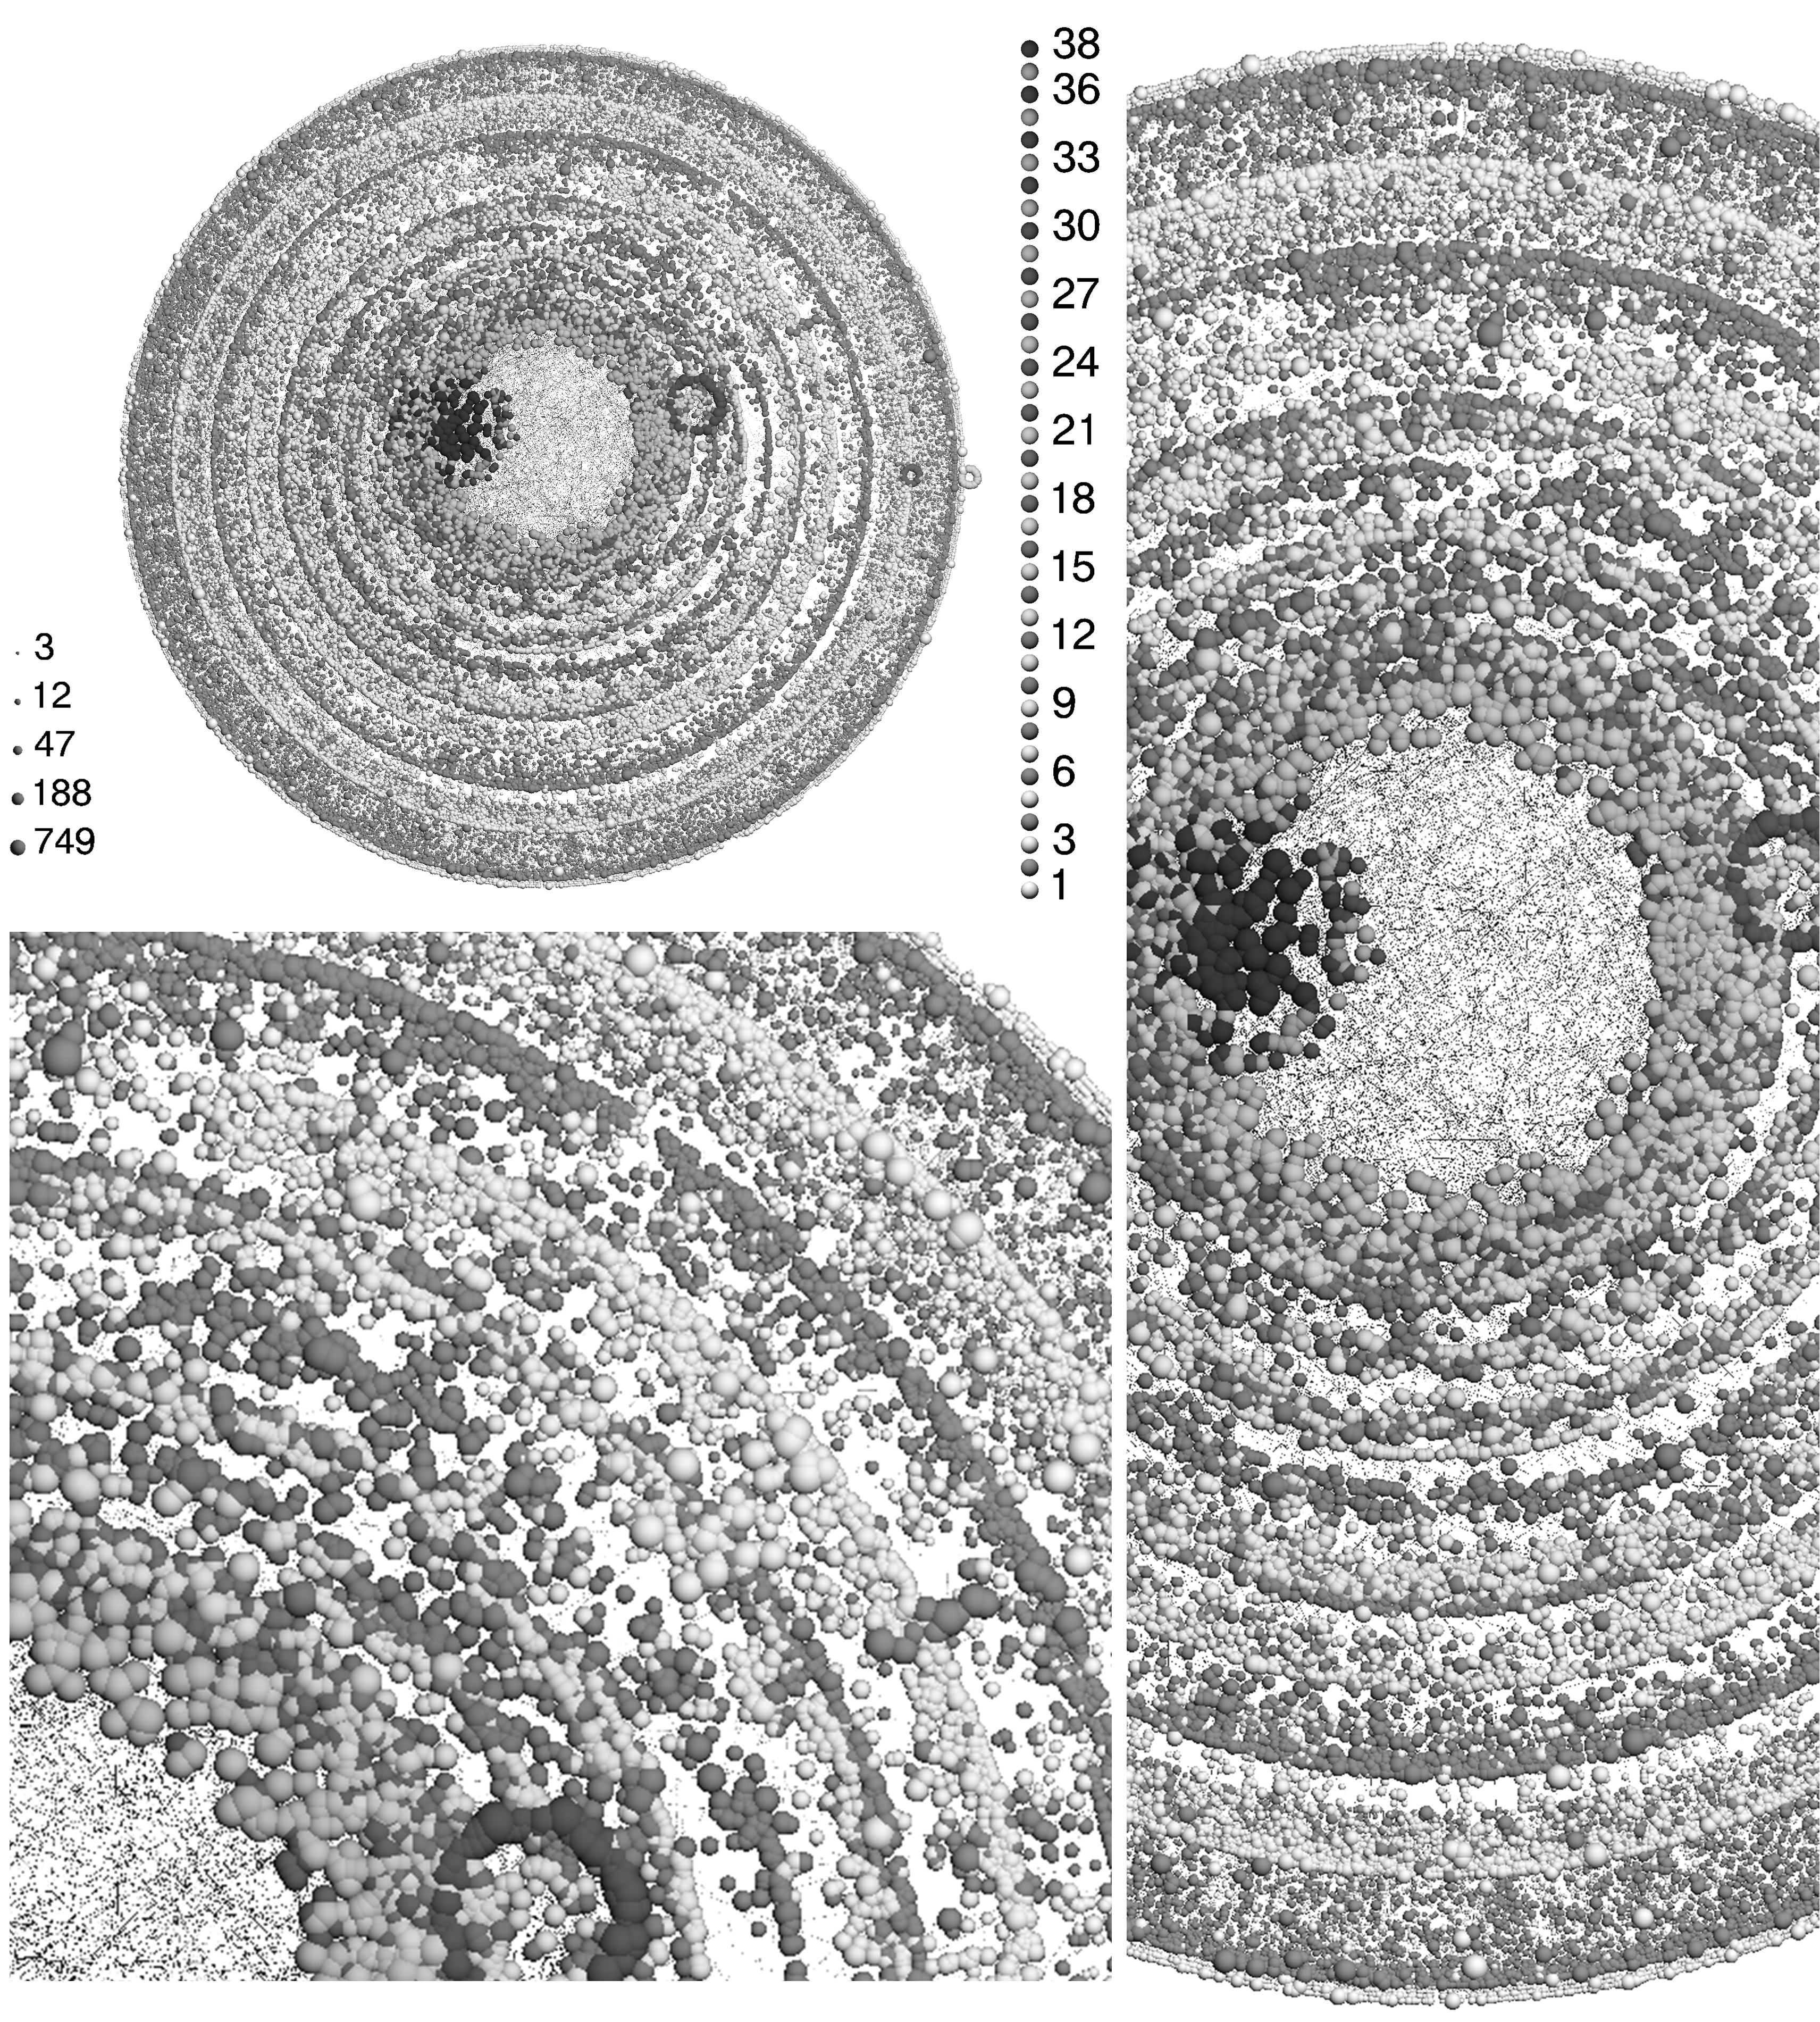
\includegraphics[width=3in]{Routers}
  \end{center}
  \caption{$k$-core visualization of router level topology $G_{r}$.}
  \label{fig_k_core_routers}
\end{figure}

We first analyze the graphs $G_{ip}$ and $G_{r}$ in order to know if there are
some strong differences between their structure and properties. As expected, we
notice that the router level topology has slightly stronger clustering
coefficient than the IP level topology (see Fig.~\ref{fig_clustering}), due to
% the join of IP interfaces into single routers.
alias resolution process.  However, the main structure of both topologies iss
similar as displayed on Fig.~\ref{fig_degree_distribution}
and~\ref{fig_neighbor}. Because we do not see any meaningful difference
between these topologies, and the router level topology is closer to a
realistic Internet one, we use the later for the remaining of our analysis.

Fig.~\ref{fig_k_core_routers} shows the $k$-core visualization of $G_{r}$.  The
figure is divided in three parts, the main part being in the upper left while
the two others are a zoom on the main part.  The main part is composed of two
scales, the one on the left is the node degree scale representing the degree in
a logarithmic scale, while the one on the right is a gray scale with each shell
index $c_i$.  Between the two scales, we see the shell index with $C_{\max}$ in
the center, the other shells being located concentrically around it. Note that
$C_{\max}$-core is made of several components with one having the most
significant part, and it is shown at the left of the center (black nodes).  We
also see that all the shells index are highly populated and that the node degree
is not related with the shell index, i.e., there are many routers with high
degree in the outer (lower) shells.  Another typical feature of router level
topology is that the links between routers mainly occurs between routers
belonging to neighbors shells, e.g., the routers on the outer shells are not
usually connected to the routers located on the  $C_{\max}$-core, as it is in
the Autonomous Systems maps~\cite{Alvarez06k}.

\begin{figure*}[!t]
  \begin{center}
    \subfigure[The $k$-core visualization of router level topology $G_{r}$.]{\label{fig_k_core_LSR}
      \includegraphics[width=18cm]{LSR}}
\hfil
    \subfigure[The $k$-core visualization of MPLS cluster level topology  $G_{r\backslash lsr}$.]{\label{fig_k_core_MPLS}
      \includegraphics[width=18cm]{MPLS}}
  \end{center}
  \caption{$k$-core visualization of $G_r$ and $G_{r \backslash lsr}$.  On
  Fig.~\ref{fig_k_core_LSR}, black nodes refer to non MPLS capable routers and
  gray nodes refer to LSRs.  On Fig.~\ref{fig_k_core_MPLS}, black nodes refer to
  non MPLS capable routers and gray nodes refer to MPLS clusters.} 
  \label{fig_kcore_overview}
\end{figure*}

In order to locate LSRs-routers with MPLS capabilities into the shells index
over $k$-core decomposition, we paint in black the non-MPLS routers and in gray
the LSRs. The results are showed in Fig.~\ref{fig_k_core_LSR}.  For the sake of
the visualization, we do not include neither the shell index, degree scale, nor
edges between shells. We notice that the LSRs are commonly distributed around
the different shells of Internet but slightly tends to concentrate with more
density nearby the $C_{\max}$-core. Additionally, we apply the same methodology
for the MPLS interconnection cluster level graph $G_{r\backslash lsr}$
(Fig.~\ref{fig_k_core_MPLS}): MPLS clusters (gray nodes) are distinguished from
the non MPLS capable routers (black nodes). In this case,  MPLS clusters  are
also spread out on the Internet.  Indeed, we see some well defined gray nodes on
the periphery of the decomposition. However MPLS clusters show a stronger
tendency to concentrate near the $C_{\max}$-core.

Finally, we evaluate the impact of MPLS clusters on the typical router level
topology, i.e., MPLS cluster interconnection graph $G_{r \backslash lsr }$. We
use metrics such as degree distribution, clustering coefficient, and nearest
neighbor degree, as is shown on Fig.~\ref{fig_metrics}.
We notice that MPLS clusters highly impact over the router level topology. On
one hand, the nearest neighbor degree highly increments for low degrees nodes on
$G_{r \backslash lsr }$, suggesting that routers with low degree are highly
connected to MPLS clusters and thereby to LSRs. On the other hand, the
clustering coefficient of $G_{r \backslash lsr }$ change significantly their
slope in regards with IP and router level topology, indicating that routers with
high degree are connected to \textit{common} MPLS clusters. \ed{does this
suggest that some MPLS clusters are more ``popular'' than others?}

\subsection{\textit{MPLS clusters} on Autonomous Systems}\label{cluster.as}
% %%%%%%%%%%%%%%%%%%%%%%%%%%%%%%%%%%%%%%%%%%%%%%%%%%%%%%%%%
Although, the previous results give us a general overview about MPLS deployment,
we believe that the study of MPLS structure requires to go deeper into the
individual AS topology. Indeed, we found that around $89.9\%$ of \textit{mpls
links} are intra-domain. Thereby, we focus on the top ASes in terms of total
number of discovered links.  On this set of ASes, we discard those having less
than 500 mpls links. Additionally, we identify the amount of mpls
links by AS, distinguishing the type of tunnel \ed{unclear}:

\begin{itemize}
  \item[i] \textit{explicit mpls link:} Link between an interface
  $i^{\text{explicitMPLS}}_{n}$  and its immediate previous interface
  $i^{\text{MPLS}}_{n-1}$ discovered by traceroute, such that
  $i^{\text{explicitMPLS}}_{n}$ belongs to an explicit MPLS tunnel and
  $i^{\text{MPLS}}_{n-1}$ belongs to any kind of MPLS tunnel (explicit,
  \textit{qTTL} based or \textit{u-turn} based).
  \item[ii] \textit{qTTL mpls link:} Link between the interfaces
  $i^{\text{qTTL}}_{n}$  and $i^{\text{MPLS}}_{n-1}$, such that
  $i^{\text{qTTL}}_{n}$ belongs to a tunnel \textit{qTTL} based.
  \item[iii] \textit{u-turn mpls link:} Link between the interfaces
  $i^{\text{u-turn}}_{n}$  and $i^{\text{MPLS}}_{n-1}$, such that
  $i^{\text{u-turn}}_{n}$ belongs to a tunnel \textit{u-turn} based.
\end{itemize}

The summary of the top ASes is showed in the Fig.~\ref{top_as}.
We noticed that the ratio $r_{mpls}= \vert E^{mpls}_{r} (as) \vert /\vert E_{r}
(as) \vert $  is greater when more  \textit{explicit mpls links} have been
discovered. Interestingly, we also see that the ASes with more links discovered
have the lowest ratio $r_{mpls}$.

For our purposes, we select the most representatives ASes from those in
Fig.~\ref{top_as}. In this way we analyzed the graphs $G_{r}(as)$ and
$G_{r\backslash lsr}(as)$ for AS1299, AS174, AS6762, AS7018, AS1273 and AS2914.
The most remarkable observation (see Fig.~\ref{fig_cluster_mpls}) occurs
regarding the graph $G_{r\backslash lsr}(as)$: $k$-core decomposition highly
differs on those ASes, where prevails explicit tunnels in regard to those with
more \textit{u-turn} tunnels proportionally .We show that \textit{MPLS clusters}
(represented as gray nodes) for  AS1299 (Teliasonera AB), AS174 (Cogent
Communication) and AS6762 (Telecom Italia) are spread out over different shells
index. These $k$-core structures are similar in our top four of ASes where we
additionally noticed  the \textit{u-turn} signature was majority discovered,
i.e., between $30\%$ and  $80\%$ over  the total amount of \textit{mpls links}.
However, for AS7018 (AT\&T), AS1273 (Cable and Wireless Worldwide plc) and
AS2914 (NTT America Inc.)  where prevail explicit tunnels, we found a $k$-core
structure highly different. In these cases,  the ASes have few and well defined
\textit{MPLS clusters}, mainly belonging to the $C_{\max}$-core.
The same $k$-core decomposition structure was noticed  on the rest of top ASes
with high percentage of \textit{qTTL} signature, i.e., AS7018, AS1273 and
AS2914.

Another remarkable observation  relays on the fact that the maximum degree
reached by \textit{MPLS clusters} is considerably high in regard to the network
size. Indeed, with exception of AS174, the rest of ASes suggest that more than
$50\%$ of non mpls routers are connected  to at least one LSR. Actually, even
the outer shells of the $k$-core decomposition are linked directly with the
\textit{MPLS clusters} located in the $C_{\max}$-core. This behavior match with
our observation of nearest neighbor degree and clustering coefficient noticed on
Sec.~\ref{cluster.topo}. Additionally, because \textit{MPLS clusters} are
mainly located on $C_{\max}$-core (even on the ASes with high percentage of
\textit{u-turn mpls links}), we believe that MPLS plays an important role in the
backbone of the ISPs.

Summarizing, we observed that  $k$-core decomposition structure varies according
the type of MPLS tunnels that prevails in the AS. This observation could suggest
that exists a great number of MPLS links non revealed by \traceroute in the ASes
where prevail \textit{u-turn} signatures; therefore, the LSRs discovered can not
build large \textit{MPLS clusters} so they are thoroughly spread out.
Additionally, because \textit{u-turn} signatures are inaccurate, as we showed
previously, there could exists several false LSRs spread out over the shell
indexes, adding false \textit{MPLS clusters}. Finally, it draws our attention
that the ratio of \textit{u-turn links} differs greatly just on ASes with low
$r_{mpls}$, producing a \textit{u-turn} bias in some ASes while not in others,
yielding inaccuracies to topology.


\begin{figure}[!htb]
  \begin{center}
    \includegraphics[width=8cm]{TOP_AS}
  \end{center}
  \caption{Top of ASes with most links discovered} On top four ASes
  prevails \textit{u-turn mpls links}. On the rest of ASes prevails \textit{qttl
  mpls links.}
  \label{top_as}
\end{figure}

%Figura u-turn
\begin{figure*}[!htb]
  \begin{center}
    \subfigure[AS1299  Teliasonera AB , $C_{\max}=21$, $\text{Degree}_{\max}=2781$]{\label{fig_cluster_mpls_1299}
      \includegraphics[width=2in]{1299}}
\hfill
    \subfigure[AS174 Cogent Communication, $C_{\max}=8$, $\text{Degree}_{\max}=751$]{\label{fig_cluster_mpls_174}
      \includegraphics[width=2in]{174}}
\hfill
    \subfigure[AS6762 Telecom Italia, $C_{\max}=10$, $\text{Degree}_{\max}=564$]{\label{fig_cluster_mpls_6762}
      \includegraphics[width=2in]{6762}}
\hfill
    \subfigure[AS7018 AT\&T, $C_{\max}=3$, $\text{Degree}_{\max}=745$]{\label{fig_cluster_mpls_2914}
      \includegraphics[width=2in]{2914}}
\hfil
    \subfigure[ AS1273 Cable and Wireless Worldwide plc, $C_{\max}=3$, $\text{Degree}_{\max}=806$]{\label{fig_cluster_mpls_1273}
      \includegraphics[width=2in]{1273}}
\hfil
    \subfigure[AS2914 Citicorp, $C_{\max}=4$, $\text{Degree}_{\max}=745$]{\label{fig_cluster_mpls_7018}
      \includegraphics[width=2in]{7018}}
  \end{center}
  \caption{$k$-core visualization of MPLS cluster interconnection Graph
  $G_{r\backslash lsr}(as)$. On the top the ASes show \textit{MPLS clusters}
  spread out around the shell index of the decomposition. On the bottom the ASes
  show \textit{MPLS clusters} well defined and located on the top core
  $C_{\max}$.}
  \label{fig_cluster_mpls}
\end{figure*}
\section{Conclusion}\label{ccl}
%%%%%%%%%%%%%%%%%%%%
remind the higher interest of MPLS within the research community (while there
are still many things to explore for MPLS).

remind our approaches and our main results

potentially, provide insight for future research directions.

\section*{Acknowledgments}\label{ack}
%%%%%%%%%%%%%%%%%%%%%%%%%%
This work is partially funded by the European Commission funded mPlane
ICT-318627 project, and also by UBACyT 2014 (20020130200122BA).


{\small
 \bibliographystyle{IEEEtran}
 \bibliography{IEEEabrv,Bibliography}
}

\end{document}
